
%(BEGIN_QUESTION)
% Copyright 2009, Tony R. Kuphaldt, released under the Creative Commons Attribution License (v 1.0)
% This means you may do almost anything with this work of mine, so long as you give me proper credit

Calculate and superimpose two different {\it load lines} on top of the transistor's characteristic curves, one load line assuming a 2 k$\Omega$ collector (load) resistor, and another assuming no collector resistor at all (i.e. a constant 20 volts between collector and emitter at all times):

$$\includegraphics[width=15.5cm]{i01386x01.eps}$$

\vfil \eject

Now, plot two graphs showing the relationship between base current ($I_B$) and collector current ($I_B$), one graph for each load condition (no load resistor versus a 2 k$\Omega$ load resistor).  In which case is the relationship between base and collector current more linear?  Explain why.

$$\includegraphics[width=15.5cm]{i01386x03.eps}$$

Also, explain how this electronic circuit's behavior relates to the installed versus inherent characteristics of control valves.  Identify what each of these parameters in the transistor circuit is analogous to in a control valve scenario:

\begin{itemize}
\item{} Base current
\item{} Collector current
\item{} Collector-emitter voltage 
\item{} Collector resistor (load) value
\end{itemize}

\underbar{file i01386}
%(END_QUESTION)





%(BEGIN_ANSWER)

The two load lines are shown here, superimposed on the same characteristic curve graph:

$$\includegraphics[width=15.5cm]{i01386x02.eps}$$

\vskip 10pt

$$\hbox{No load resistor \hskip 70pt 2 k$\Omega$ load resistor}$$

% No blank lines allowed between lines of an \halign structure!
% I use comments (%) instead, so that TeX doesn't choke.

$$\vbox{\offinterlineskip
\halign{\strut
\vrule \quad\hfil # \ \hfil & 
\vrule \quad\hfil # \ \hfil \vrule \cr
\noalign{\hrule}
%
% First row
$I_B$ & $I_C$ \cr
%
\noalign{\hrule}
%
% Another row
10 $\mu$A & 1.4 mA \cr
%
\noalign{\hrule}
%
% Another row
20 $\mu$A & 2.9 mA \cr
%
\noalign{\hrule}
%
% Another row
30 $\mu$A & 4.4 mA \cr
%
\noalign{\hrule}
%
% Another row
40 $\mu$A & 5.8 mA \cr
%
\noalign{\hrule}
%
% Another row
50 $\mu$A & 7.25 mA \cr
%
\noalign{\hrule}
%
% Another row
60 $\mu$A & 8.7 mA \cr
%
\noalign{\hrule}
%
% Another row
70 $\mu$A & 10.1 mA \cr
%
\noalign{\hrule}
%
% Another row
80 $\mu$A & 11.6 mA \cr
%
\noalign{\hrule}
%
% Another row
90 $\mu$A & 13.1 mA \cr
%
\noalign{\hrule}
%
% Another row
100 $\mu$A & 14.5 mA \cr
%
\noalign{\hrule}
} % End of \halign 
}
\hskip 40pt
\vbox{\offinterlineskip
\halign{\strut
\vrule \quad\hfil # \ \hfil & 
\vrule \quad\hfil # \ \hfil \vrule \cr
\noalign{\hrule}
%
% First row
$I_B$ & $I_C$ \cr
%
\noalign{\hrule}
%
% Another row
10 $\mu$A & 1.4 mA \cr
%
\noalign{\hrule}
%
% Another row
20 $\mu$A & 2.6 mA \cr
%
\noalign{\hrule}
%
% Another row
30 $\mu$A & 3.75 mA \cr
%
\noalign{\hrule}
%
% Another row
40 $\mu$A & 4.8 mA \cr
%
\noalign{\hrule}
%
% Another row
50 $\mu$A & 5.75 mA \cr
%
\noalign{\hrule}
%
% Another row
60 $\mu$A & 6.7 mA \cr
%
\noalign{\hrule}
%
% Another row
70 $\mu$A & 7.5 mA \cr
%
\noalign{\hrule}
%
% Another row
80 $\mu$A & 8.25 mA \cr
%
\noalign{\hrule}
%
% Another row
90 $\mu$A & 9 mA \cr
%
\noalign{\hrule}
%
% Another row
100 $\mu$A & 9.4 mA \cr
%
\noalign{\hrule}
} % End of \halign 
}
$$ % End of \vbox

\vskip 10pt

\filbreak

The analogous quantities between the transistor circuit and the control valve installation are as follows:

\begin{itemize}
\item{} Base current = {\it $C_v$ value, which is directly proportional to stem position for a linear control valve trim}
\item{} Collector current = {\it flow ($Q$) through the valve}
\item{} Collector-emitter voltage = {\it pressure drop ($P_1 - P_2$) across the valve}
\item{} Collector resistor (load) value = {\it pressure losses due to flow through pipes, exchangers, pumps, etc.}
\end{itemize}

$$\includegraphics[width=15.5cm]{i01386x04.eps}$$

Superimposing a linear function on top of a set of nonlinear functions and looking for the intersection points allows us to solve for multiple variables in a nonlinear mathematical system.  Normally, only {\it linear} systems of equations are considered ``solvable'' without resorting to very time-consuming arithmetic computations, but here we have a powerful (graphical) tool for approximating the values of variables in a nonlinear system.  Since approximations are the best we can hope for in transistor circuits anyway, this is good enough!


%(END_ANSWER)





%(BEGIN_NOTES)


%INDEX% Electronics review: load lines
%INDEX% Final Control Elements, valve: characterization

%(END_NOTES)


